\section{System Design}
\label{sec:design}

\noindent
This section answers the three coupled sub-problems raised in
\autoref{sec:bg-motivation:implications}, layer by layer:
\autoref{sec:design:controller} derives a stable~$S_t$ from partial
observations; \autoref{sec:design:forecaster} predicts the experts
needed over the next~$S_t$ layers without consuming GPU cycles; and
\autoref{sec:design:memory} bounds the cost of misprediction so that
errors cause at most one DMA, never a cascade of stalls. We start
with the system overview that ties them together
(\autoref{sec:design:overview}).

\subsection{Overview and Architecture}
\label{sec:design:overview}

\systemname\ converts MoE inference into a closed-loop scheduling
problem over a single scalar~$S_t$. The system has three layers
(\autoref{fig:architecture}). The \emph{controller}
(\autoref{sec:design:controller}) updates~$S_t$ from EMA-smoothed
runtime signals at constant per-update cost. The \emph{forecaster}
(\autoref{sec:design:forecaster}) predicts the experts likely to be
activated over the next~$S_t$ layers using token-, layer-, and
horizon-aware features, on the CPU. The \emph{memory layer}
(\autoref{sec:design:memory}) materializes the forecast through
asynchronous transfers, a two-tier cache that protects high-reuse
experts, and cache-aware token routing that lets cache misses be
absorbed in parallel with resident-expert execution.

\begin{figure}
    \centering
    {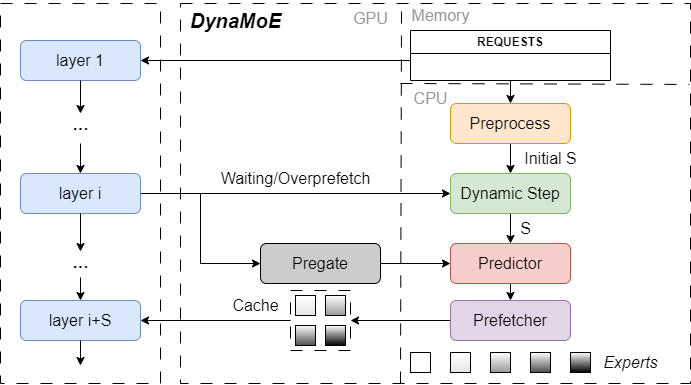
\includegraphics[width=0.99\linewidth]{figures/architecture.png}}
    \vspace{-0.5em}
    \caption{Architecture of \systemname.
    \emph{Online path:}
    (1)~per-layer hooks read smoothed waiting and miss signals
    $(\tilde{w}_t,\tilde{m}_t)$;
    (2)~the controller updates the horizon~$S_t$
    (\autoref{alg:controller});
    (3)~the forecaster emits the expert set $\hat{E}_{\ell+1..\ell+S_t}$
    and a confidence score;
    (4)~the two-tier cache issues asynchronous prefetches for
    non-resident experts on a dedicated transfer stream;
    (5)~the cache-aware router executes tokens whose experts are
    already resident first, deferring the rest until prefetch
    completes.
    \emph{Offline path:} the forecaster's CPU-side random forest is
    trained from logged $(\mathbf{t},\ell,S,\mathbf{a})$ tuples; no GPU
    cycles are spent on prediction at serving time.}
    \label{fig:architecture}
\end{figure}

Each control period~$T_u$, the controller solves the following
optimization:
\begin{equation}
\label{eq:formulation}
\begin{aligned}
\min_{S_{t+1}\in\mathbb{Z}\cap[S_{\min},S_{\max}]} \;
   & \tilde{L}_{\text{wait}}(S_{t+1}) + \lambda\,\tilde{L}_{\text{miss}}(S_{t+1}), \\[-1pt]
\text{s.t.}\quad
   & \text{(C1)}\;\mathrm{occ}(\hat{E}_{\ell+1..\ell+S_{t+1}})\le M_{\text{HBM}}, \\[-1pt]
   & \text{(C2)}\;|S_{t+1}-S_t|\le 1, \\[-1pt]
   & \text{(C3)}\;\text{prefetch}\subseteq\hat{E}_{\ell+1..\ell+S_{t+1}}.
\end{aligned}
\end{equation}
$\tilde{L}_{\text{wait}}$ and $\tilde{L}_{\text{miss}}$ are
EMA-smoothed exposed-stall and eviction-pressure proxies
(\autoref{sec:design:controller}); $\hat{E}$ is the forecaster's
prediction (\autoref{sec:design:forecaster}); $M_{\text{HBM}}$ is the
expert residency budget. (C1) keeps each candidate~$S$ realizable
under the HBM cap, (C2) bounds per-step change so the controller
cannot oscillate, and (C3) keeps speculative prefetching restricted
to the current prediction set. \systemname\ exposes only two scalar
hyperparameters---the regime weight~$\lambda$ and the hysteresis
threshold~$\theta_h$ used by the controller---both fixed once at
startup.

The rest of this section answers, in order:
\begin{itemize}[leftmargin=1.4em, itemsep=2pt, topsep=2pt]
    \item \textbf{Q1.}\,How can the controller pick a stable~$S_t$ from
    partial, noisy observations of bandwidth, demand, and cache state?
    (\autoref{sec:design:controller})
    \item \textbf{Q2.}\,How can a predictor extend pregate signals over
    long horizons without competing for GPU cycles?
    (\autoref{sec:design:forecaster})
    \item \textbf{Q3.}\,How can the memory layer bound the cost of
    misprediction so that errors cause at most one DMA, never a
    cascade of stalls? (\autoref{sec:design:memory})
\end{itemize}

\subsection{Adaptive Controller}
\label{sec:design:controller}

The controller maintains EMA-smoothed estimates of two runtime
signals: $\tilde{w}_t = \mathrm{EMA}_\alpha(w_t)$ for exposed waiting
(the fraction of MoE-layer time spent stalled on a missing expert)
and $\tilde{m}_t = \mathrm{EMA}_\alpha(m_t)$ for pollution pressure
(evictions per miss-induced refill). Smoothing decouples the
controller from per-layer noise without introducing learned state.
The signed quantity $\Delta_t = \tilde{w}_t - \lambda\,\tilde{m}_t$
identifies the dominant failure mode at each control period:
$\Delta_t > 0$ means waiting dominates (under-prefetch), $\Delta_t < 0$
means pollution dominates (over-prefetch); the weight $\lambda$ trades
off the two costs, and we use $\lambda = 1$ throughout this paper.

The controller updates~$S$ by at most one layer per period inside a
hysteresis band of width~$\theta_h$:
$S_{t+1} = \min(S_t{+}1, S_{\max})$ if $\Delta_t > \theta_h$;
$\max(S_t{-}1, S_{\min})$ if $\Delta_t < -\theta_h$; and $S_t$
otherwise. The rule satisfies constraint~(C2) of
\autoref{eq:formulation} by construction. A short informal argument
explains stability. Inside the band the rule is the identity, so once
the regime indicator enters the band, $S_t$ is fixed. Outside the
band, $|\Delta_t|>\theta_h$ deterministically pushes $S_t$ toward the
regime knee at one layer per period; bounded by
$[S_{\min}, S_{\max}]$, the trajectory reaches a band-boundary in at
most $S_{\max}-S_{\min}$ periods. EMA smoothing ($\alpha\in[0,1)$)
exponentially attenuates the indicator's response to any single noisy
observation, so the controller cannot be flipped in and out of the
band by a transient spike.

\autoref{alg:controller} summarizes one control period. The per-update
cost is $O(1)$; the aggregate per-request cost is
$O(L_{\text{MoE}})$, independent of model size, batch size, and~$S$.
An update completes in under $50\,\mu$s on a commodity CPU in our
implementation. Lines~1--2 update the smoothed signals; line~3
computes $\Delta_t$; lines~4--10 are the $\pm 1$ rule above. Across
one request the controller has three typical phases: in the first
periods after a workload change $\Delta_t$ is consistently outside
the band and~$S$ moves monotonically toward the new knee; around the
knee $\Delta_t$ enters the band and~$S$ holds; under sustained drift
(a co-tenant traffic spike, or a batch with very different
intra-batch dispersion) $\Delta_t$ leaves the band again and the
controller re-converges.

Before any feedback is available, $S$ is initialized from a coarse
analytical estimate using forecaster output and recent transfer
timing. With $N_e$ predicted experts per layer of size $E_s$ bytes,
measured effective bandwidth $C_s$, and per-layer compute time $T_l$,
the transfer of one layer's experts takes $N_e E_s / C_s$ seconds,
which the controller hides behind $S\cdot T_l$ seconds of compute.
Solving for $S$ gives
\(
S_0 = \lceil N_e E_s / (C_s T_l) \rceil,
\)
in units of MoE layers. The closed-loop rule then takes over at the
first control period; mis-set $S_0$ only delays convergence.

\begin{algorithm}[t]
\caption{\systemname\ adaptive horizon controller (per control period~$T_u$).}
\label{alg:controller}
\begin{algorithmic}[1]
\Require EMA factor $\alpha$, regime weight $\lambda$, hysteresis $\theta_h$, bounds $[S_{\min}, S_{\max}]$
\Require previous state $(\tilde{w}_{t-1}, \tilde{m}_{t-1}, S_t)$, raw counters $w_t, m_t$
\Ensure next horizon $S_{t+1}$
\State $\tilde{w}_t \gets \alpha\,\tilde{w}_{t-1} + (1-\alpha)\,w_t$ \Comment{smoothed waiting}
\State $\tilde{m}_t \gets \alpha\,\tilde{m}_{t-1} + (1-\alpha)\,m_t$ \Comment{smoothed pollution}
\State $\Delta_t \gets \tilde{w}_t - \lambda\,\tilde{m}_t$         \Comment{regime indicator}
\If{$\Delta_t > \theta_h$}                                         \Comment{stall-dominated}
    \State $S_{t+1} \gets \min(S_t + 1,\, S_{\max})$
\ElsIf{$\Delta_t < -\theta_h$}                                     \Comment{pollution-dominated}
    \State $S_{t+1} \gets \max(S_t - 1,\, S_{\min})$
\Else                                                              \Comment{within hysteresis band}
    \State $S_{t+1} \gets S_t$
\EndIf
\State \Return $S_{t+1}$
\end{algorithmic}
\end{algorithm}

\subsection{Forecasting Layer}
\label{sec:design:forecaster}

For each request \systemname\ logs a tuple
$(\mathbf{t}_i, \ell_i, \mathbf{p}_i, \mathbf{a}_i, s_i)$ per MoE
layer, recording token IDs, layer index, pregate-predicted experts,
actually activated experts, and the step size in effect. Tokens are
embedded through a frozen table $\mathbf{E}\in\mathbb{R}^{V\times d}$
and mean-pooled into a request descriptor
$\mathbf{e}=\tfrac{1}{k}\sum_{i=1}^k \mathbf{E}_{t_i}$; the per-layer
feature $\mathbf{x} = [\mathbf{e},\, S,\, \ell,\, \text{prev\_act}]$
concatenates this descriptor with the current horizon, layer index,
and a binary vector of prior-layer activations. A CPU-side random
forest regresses $\mathbf{x}$ to the multi-hot label $\mathbf{y}$ of
actually activated experts under MSE. We chose a forest over a deep
predictor for three system-level reasons: it adds no GPU interference,
its prediction latency at control-period granularity is sub-millisecond
on commodity CPUs and never blocks the inference critical path, and
its accuracy is stable across our model groups
(\autoref{sec:evaluation}).

Raw pregate outputs exhibit layer-local noise. The forecaster learns
the deviation $\Delta$ between pregate predictions and actual
activations and produces a refined prediction
$\hat{\mathbf{y}} = \mathbf{p} + \Delta$. When an identical
(token-sequence, layer, $S$) tuple reoccurs, the cached prediction is
reused; otherwise the system falls back to the model's own top-$k$
router logits, so \systemname\ never blocks waiting for prediction.
The forecaster passes two signals to the controller: the expected
number of experts per future layer~$N_e$ (used in $S_0$ in
\autoref{sec:design:controller}), and a confidence score derived from
historical prediction accuracy. Low confidence widens $\hat{E}$,
which tightens (C1) of \autoref{eq:formulation} and implicitly shrinks
$S$, so the controller becomes conservative when the predictor is
uncertain.

\begin{figure}[t]
    \centering
    {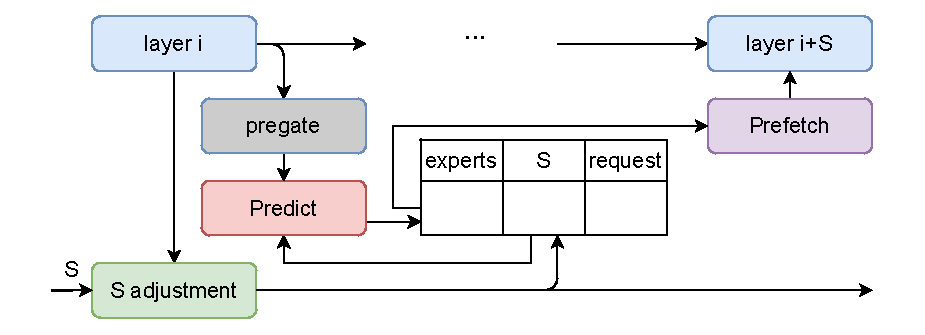
\includegraphics[width=0.99\linewidth]{figures/codesign.pdf}}
    \vspace{-0.5em}
    \caption{Co-design of the forecaster and the controller in
    \systemname. The forecaster provides $\hat{E}_{\ell+1..\ell+S}$
    and a confidence score; the controller consumes the predicted
    expert count $N_e$ to compute $S_0$ at startup, and the smoothed
    counters $\tilde{w}_t, \tilde{m}_t$ to update~$S$ at each period.
    Low-confidence forecasts widen $|\hat{E}|$, which tightens the
    HBM constraint~(C1) and implicitly shrinks~$S$, so the
    controller automatically becomes conservative when the predictor
    is uncertain.}
    \label{fig:codesign}
\end{figure}


\subsection{Expert Memory Management}
\label{sec:design:memory}

The memory layer translates forecasts into residency decisions and
returns cache statistics to the controller. It is designed so that a
mispredicted expert costs at most one extra DMA, never a cascading
stall, which is what lets the controller safely explore larger~$S$
without paying eviction--reload amplification.

\textbf{Two-tier LRU.}
Rather than a single eviction queue, \systemname\ maintains two LRU
structures: \texttt{LRU\_high} holds experts with demonstrated reuse
(recently accessed or imminently predicted), while \texttt{LRU\_low}
holds the rest. Evictions are drawn preferentially from
\texttt{LRU\_low}, which spills to host DRAM and preserves high-reuse
experts on the device. This two-tier design directly addresses a
pathology of single-tier LRU on layer-wise MoE: experts from the
first~$S$ layers are reused later during decoding, yet a single LRU
prematurely evicts them as more recent layers fill the queue.

\textbf{Prefetch--cache feedback loop.}
Memory management and the controller form a closed loop:
\textit{(1)} before computing~$S$, the controller queries current cache
occupancy to estimate effective bandwidth and the anticipated eviction
cost; \textit{(2)} after each prefetch completes, observed transfer
time updates the bandwidth estimate $C_s$ used in $S_0$
(\autoref{sec:design:controller}); \textit{(3)} cache hit/miss counters
feed $\tilde{m}_t$ in \autoref{alg:controller}. This feedback prevents
the runtime from issuing prefetches that would themselves trigger
evictions of experts the controller still expects to use.

\textbf{Cache-aware routing.}
A cache miss inside an MoE layer manifests as an asynchronous stall.
\systemname\ exploits the asynchrony by routing tokens to experts in
order of cache residency: tokens whose experts are already resident
execute first; tokens that would trigger a fault are deferred until
the corresponding swap-in completes, which happens in parallel with
the resident-expert path. Compared with conventional sequential
swap-in (where every miss blocks), this overlap reduces the exposed
component of cache-miss latency without altering routing semantics.